% !TEX root = ../presentation.tex

\subsection[Asteroid Landing]{Asteroid Landing}
\subsubsection[Coupled Dynamics]{Coupled Dynamics}

\begin{frame}{Kinematics of Dumbbell}
    \begin{itemize}
        \item Dynamics derived on \SE, Special Euclidean group
        \item Rigid dumbbell model - captures attitude coupling
        \pause
        \begin{itemize}
            \item \( \vecbf{x} \in \R^3 \) - inertial position of COM
            \item \( R \in \SO\) - transforms from body to inertial frame
            \item \( \vecbf{\Omega} \in \R^3 \) - the angular velocity of the spacecraft 
            \item \( R_A \in \SO \) - transforms from asteroid to inertial frame
        \end{itemize}    
        \pause
    \item Simple model which captures dynamic coupling  
        \begin{itemize}
            \item Models the mass distribution of spacecraft 
        \end{itemize}
        \pause
    \item Preserves the geometric properties of configuration space
    \item Attitude and Translational motion is directly coupled
\end{itemize}

\end{frame}

\begin{frame}{Equations of Motion}

    \begin{itemize}
        \item Polyhedron potential in translational and rotational dynamics
        \begin{align*}
            \dot{\vb{x}} &= \vb{v}, \\
            \parenth{m_1 + m_2} \dot{\vecbf{v}} &= m_1 R_A \deriv{U}{\vecbf{z}_1} + m_2 R_A \deriv{U}{\vecbf{z}_2} + \vecbf{u}_f, \\
            \dot{R} &= R S(\vb{\Omega}) , \\
            J \dot{\vecbf{\Omega}} + \vecbf{\Omega} \times J \vecbf{\Omega} &= \vecbf{M}_1 + \vecbf{M}_2 + \vecbf{u}_m. 
        \end{align*}
    \item Moment on dumbbell
        \begin{align*}
            \vecbf{M}_i = m_i \parenth{S(R_A^T \vb{\rho}_i) R^T \deriv{U}{\vb{z}_i}}.
        \end{align*}
    \end{itemize}
\end{frame}

\subsubsection[Geometric Control]{Geometric Control}

\begin{frame}{Nonlinear Control}
    \begin{itemize}
        \item Geometric control used to track a desired trajectory
        \item Developed directly on the nonlinear manifold
            \begin{itemize}
                \item Avoids chattering issues of sliding mode control
                \item Incorporates attitude dynamics
                \item Asymptotic trajectory tracking stability
            \end{itemize}
    \end{itemize}

\pause
\begin{align*}
    \vb{u}_m &= - k_R e_R - k_\Omega e_\Omega + \Omega \times J \Omega - J \parenth{\hat{\Omega} R^T R_d \Omega_d - R^T R_d \dot{\Omega}_d}  \\
             &- \vb{M}_1 - \vb{M_2} , \\
    \vb{u}_f &= - k_x e_x  - k_v e_v + ( m_1  + m_2 ) \ddot{x}_d - \vb{F}_1 - \vb{F}_2 
\end{align*}
\end{frame}


\begin{frame}{Landing Trajectory - Attitude}
    \begin{itemize}
        \item Goal: transition from  orbit about Itokawa to vertical descent
        \item Attitude controlled to point camera at surface
            \begin{itemize}
                \item \( \vb{b}_1 \) - body axis points at surface
                \item \( \vb{b}_3 \) - orthogonal projection in \( \vb{e}_3, \vb{b}_1\) plane
            \end{itemize}
    \end{itemize}
    \begin{columns}
        \begin{column}{0.5\textwidth}
        \begin{align*}
            \vb{b}_{1d} &= - \frac{\vb{x}}{\norm{\vb{x}}} , \\
            \vb{b}_{3d} &= \frac{\vb{f}_3 - \parenth{\vb{f}_3 \cdot \vb{b}_{1d}} \vb{b}_{1d}}{\norm{\vb{f}_3 - \parenth{\vb{f}_3 \cdot \vb{b}_{1d}} \vb{b}_{1d}}}, \\
            \vb{b}_{2d} &= \vb{b}_{3d} \times \vb{b}_{1d} , \\
        R_d &= \begin{bmatrix} \vb{b}_{1d} & \vb{b}_{2d} & \vb{b}_{3d} \end{bmatrix} .
        \end{align*}
    \end{column}
    \begin{column}{0.5\textwidth}
        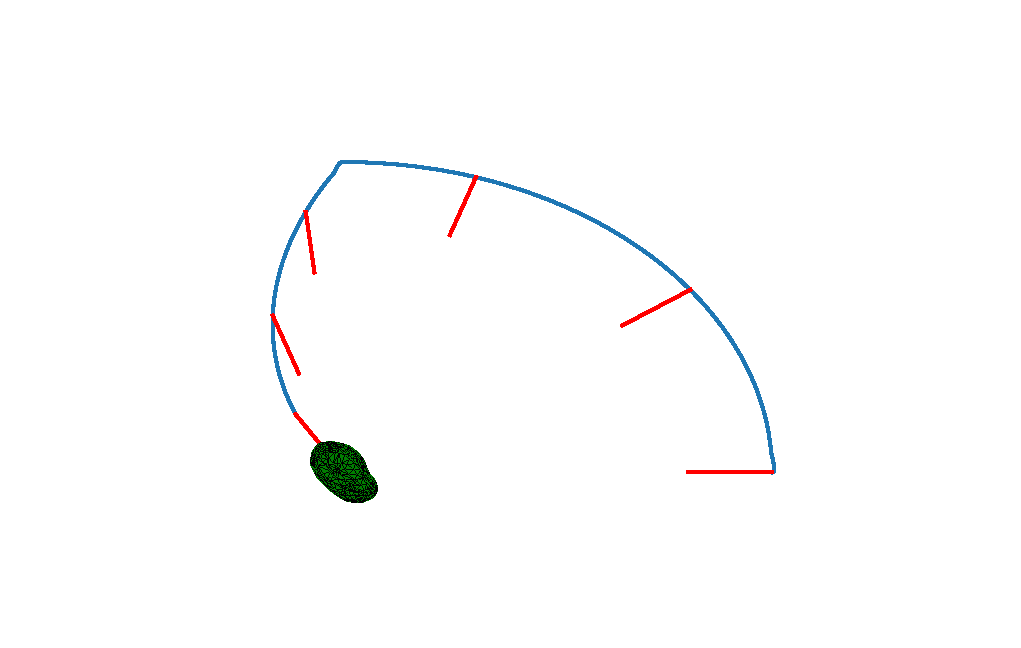
\includegraphics[width=\columnwidth,keepaspectratio,trim={30mm 20mm 30mm 20mm},clip]{figures/2017AAS_asteroid_landing/traj_fig.pdf}
\end{column}
\end{columns}
\end{frame}

\begin{frame}{Landing Trajectory - Position}
    \begin{itemize}
        \item Transition from horizontal motion to vertical descent
        \begin{itemize}
            \item Move from inertial \( \vb{e}_2 \) to asteroid \( \vb{f}_1 \) axis
            \item Remain in the equatorial plane ( \(\vb{f_1}, \vb{f}_2\) plane)
        \end{itemize}
        \pause
    \item Command is divided into two segments
        \begin{itemize}
            \item Move to \( \vb{f}_1\) along a circular path
            \item Vertical descent along \( \vb{f}_1 \)
        \end{itemize}
    \end{itemize}

    \begin{columns}
        \begin{column}{0.5\textwidth}
            \footnotesize
            \begin{align*}
                \vb{x}_d = 
                \begin{cases}
                    2.550 \begin{bmatrix} \sin{\omega t} & -\cos{\omega t} & 0 \end{bmatrix}, & t \leq t_d \\
                    R_A \begin{bmatrix} \frac{2}{t_d} (t - t_d) + 2.550 & 0 & 0 \end{bmatrix}, & t > t_d , 
                \end{cases}
            \end{align*}
        \end{column}
        \begin{column}{0.5\textwidth}
            \visible<2->{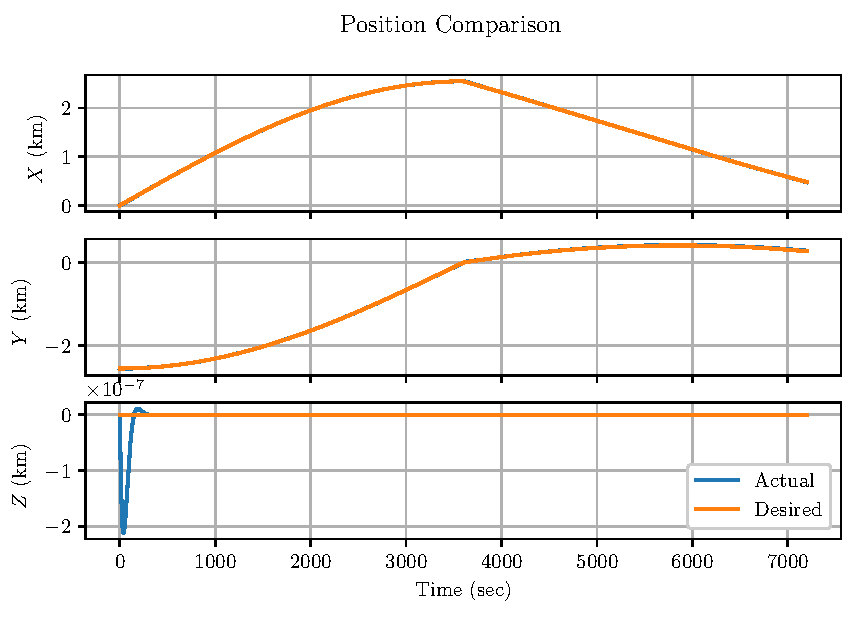
\includegraphics[width=\columnwidth]{figures/2017AAS_asteroid_landing/pos_fig.pdf}}
    \end{column}
\end{columns}
\end{frame}

\subsubsection[Image simulation]{Image Simulation}

\begin{frame}[fragile]{Blender Simulation}
    \only<1>{
    \begin{itemize}
        \item Open-source computer graphics rendering
            \begin{itemize}
                \item Photorealistic Rendering
                \item Realistic material and lighting 
                \item Physics based simulation and game engine
            \end{itemize}
        \item Additional capability by utilizing a Python API 
            \begin{itemize}
                \item Load a asteroid shape model
                \item Define camera properties/location
                \item Define light source and position
                \item Render image
            \end{itemize}
\end{itemize}

\begin{center}
    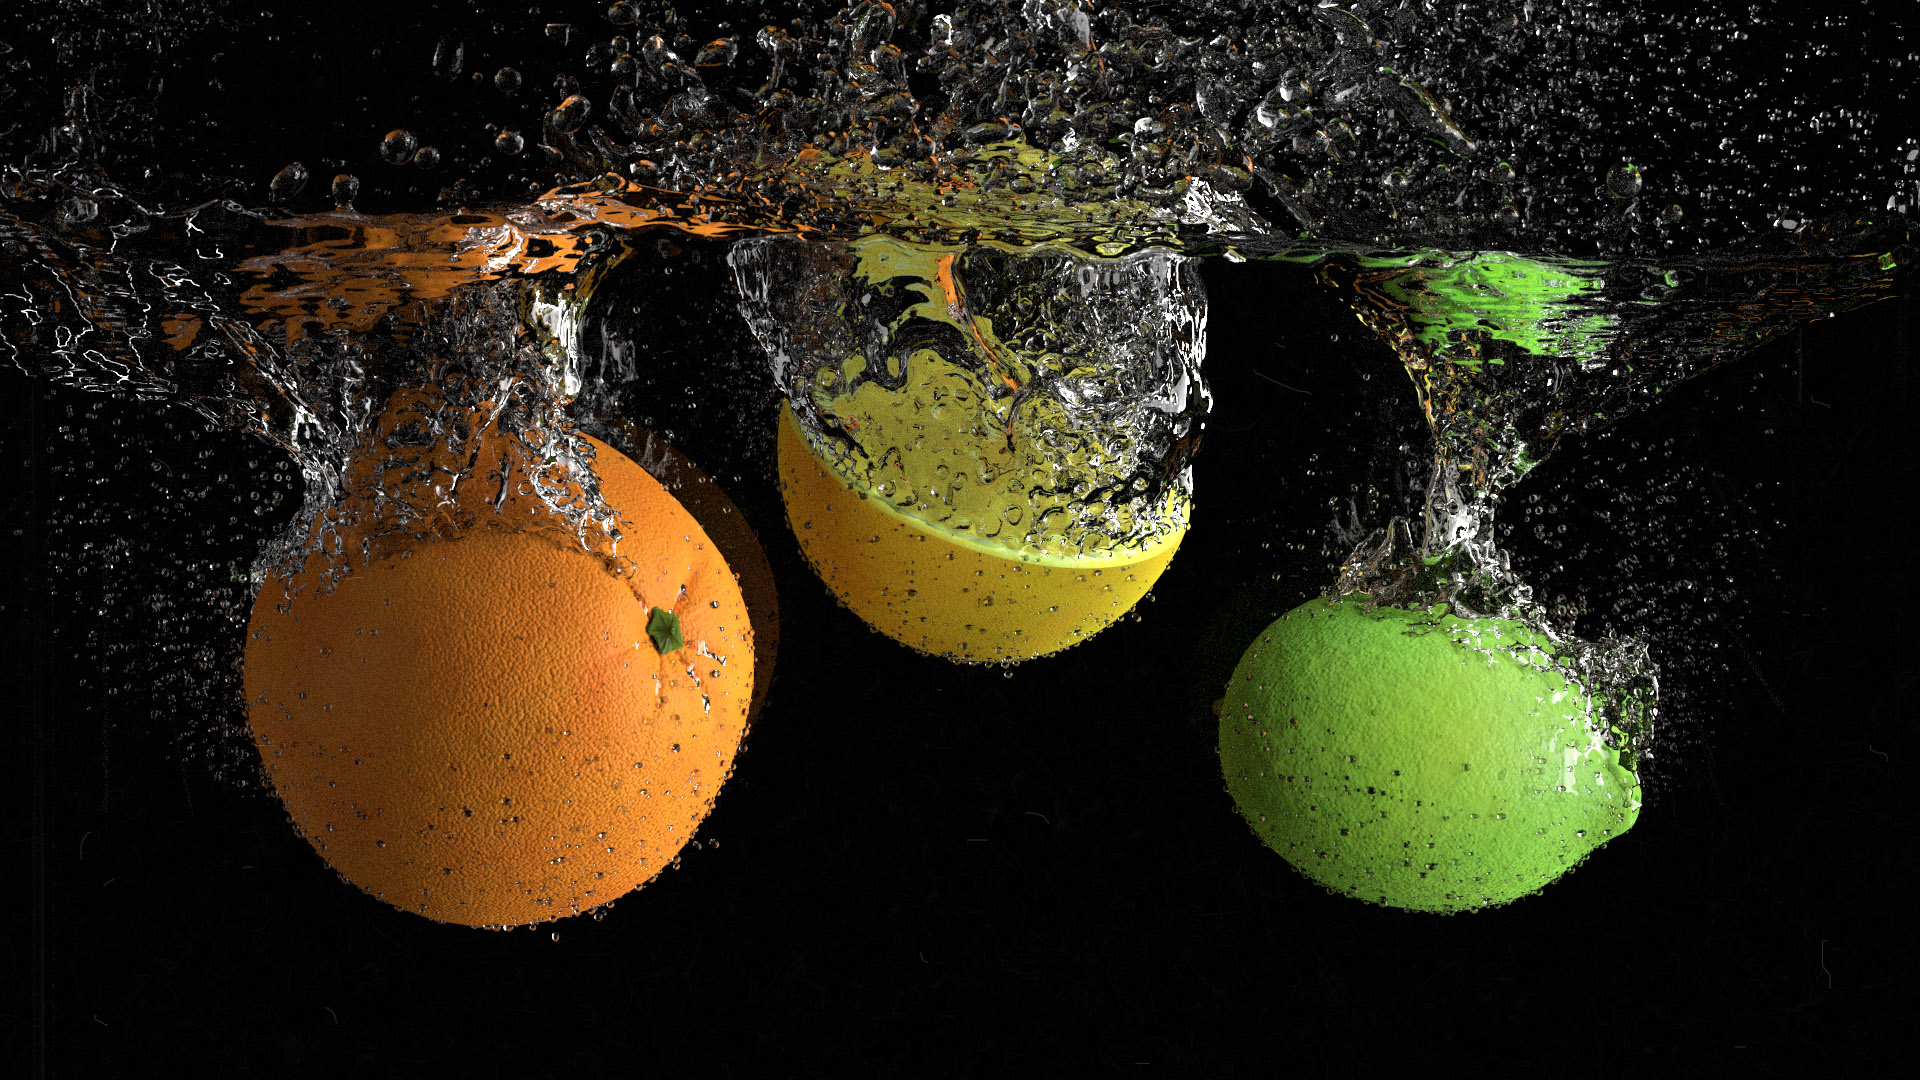
\includegraphics[width=0.5\textwidth,height=0.3\textheight,keepaspectratio]{figures/2017AAS_asteroid_landing/rendering.jpg}~
    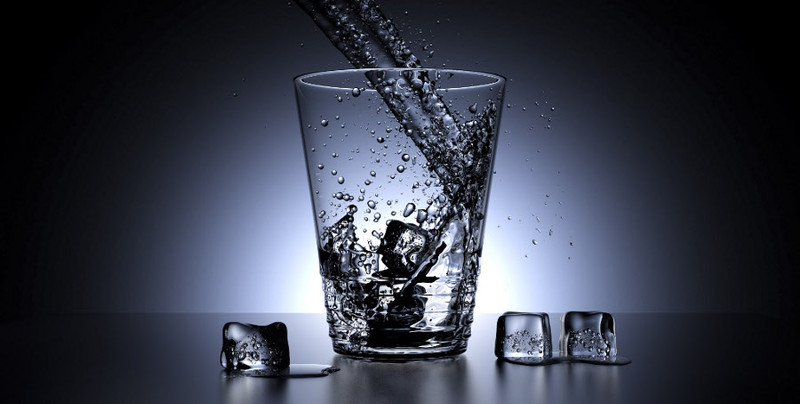
\includegraphics[width=0.5\textwidth,height=0.3\textheight,keepaspectratio]{figures/2017AAS_asteroid_landing/463e785104.jpg}
\end{center}
}

\only<2>{
    \begin{itemize}
        \item Can render scenes using a graphical interface
    \end{itemize}
    \begin{center}
        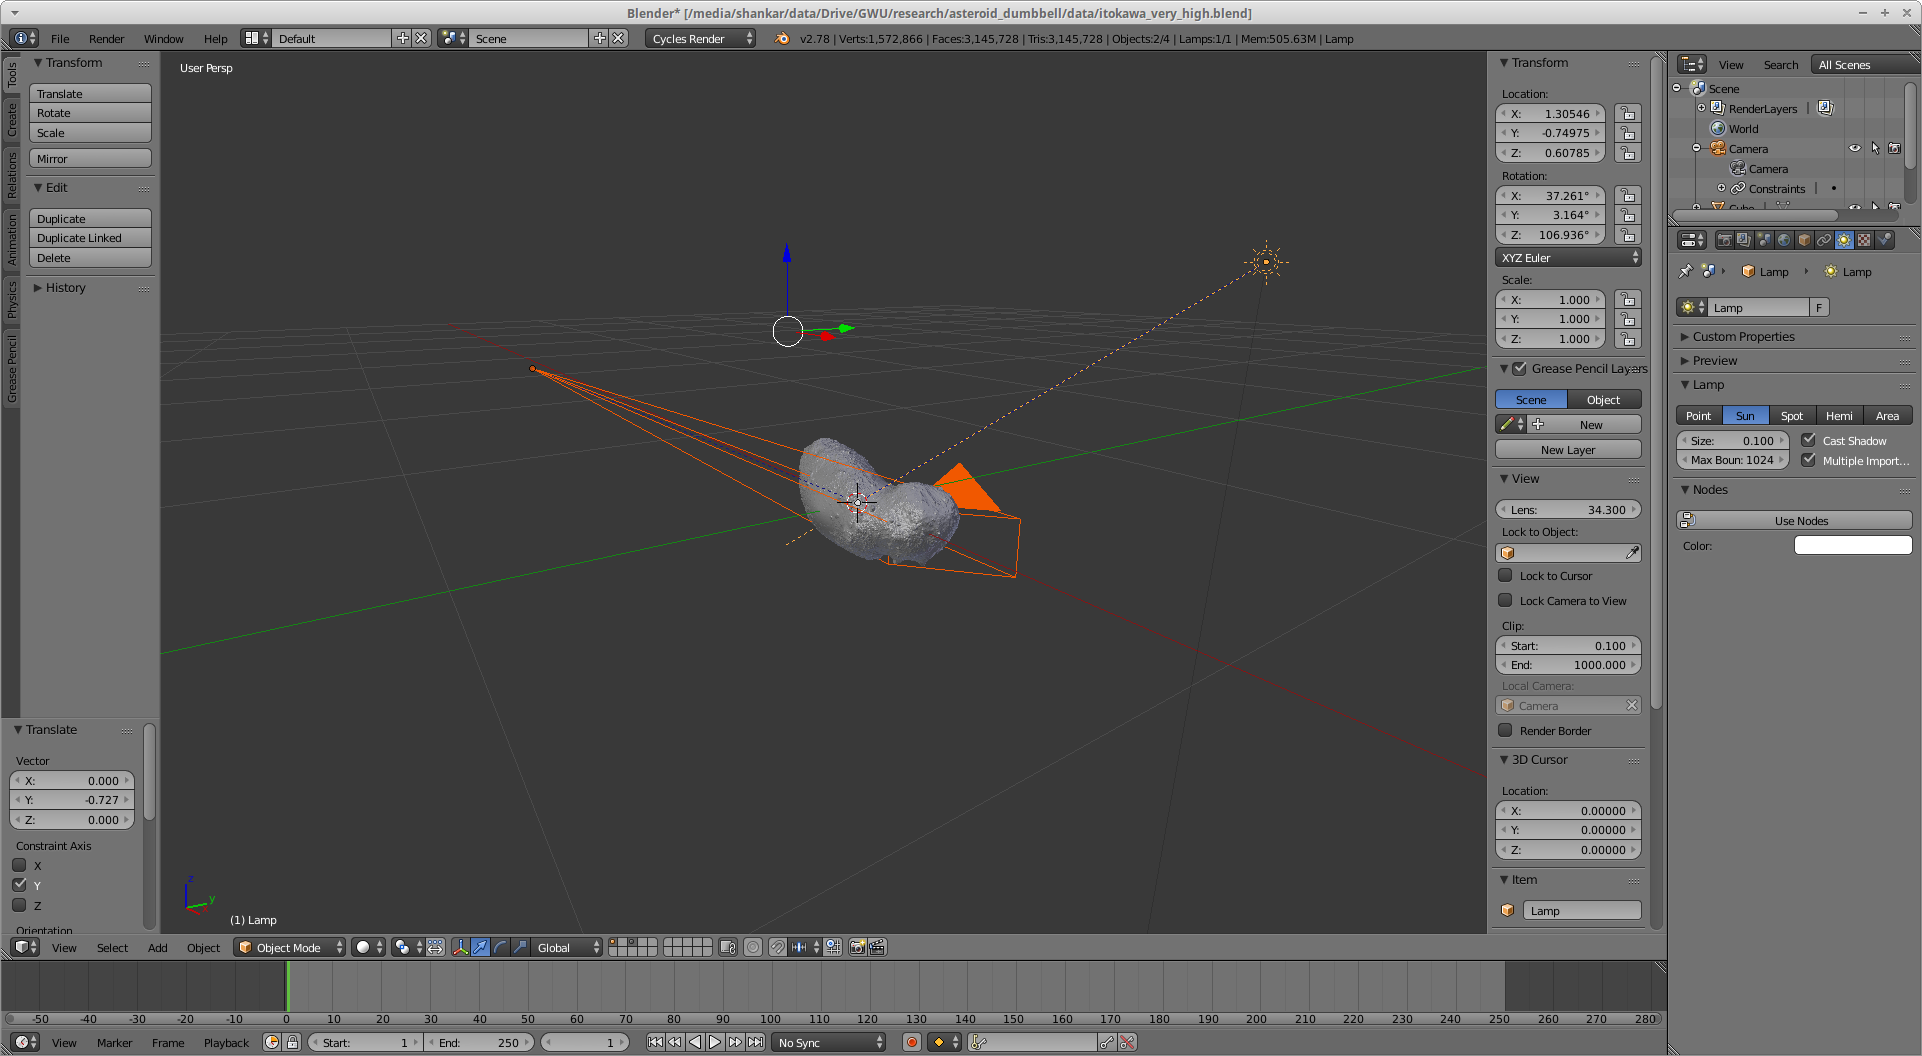
\includegraphics[height=0.8\textheight,width=\textwidth,keepaspectratio]{figures/2017AAS_asteroid_landing/blender_screenshot.png}
    \end{center}
}

\only<3>{
    \begin{itemize}
        \item Python used to generate imagery - incorporate in larger code
    \end{itemize}
    \begin{columns}
        \begin{column}{0.5\textwidth}
            \begin{center}
                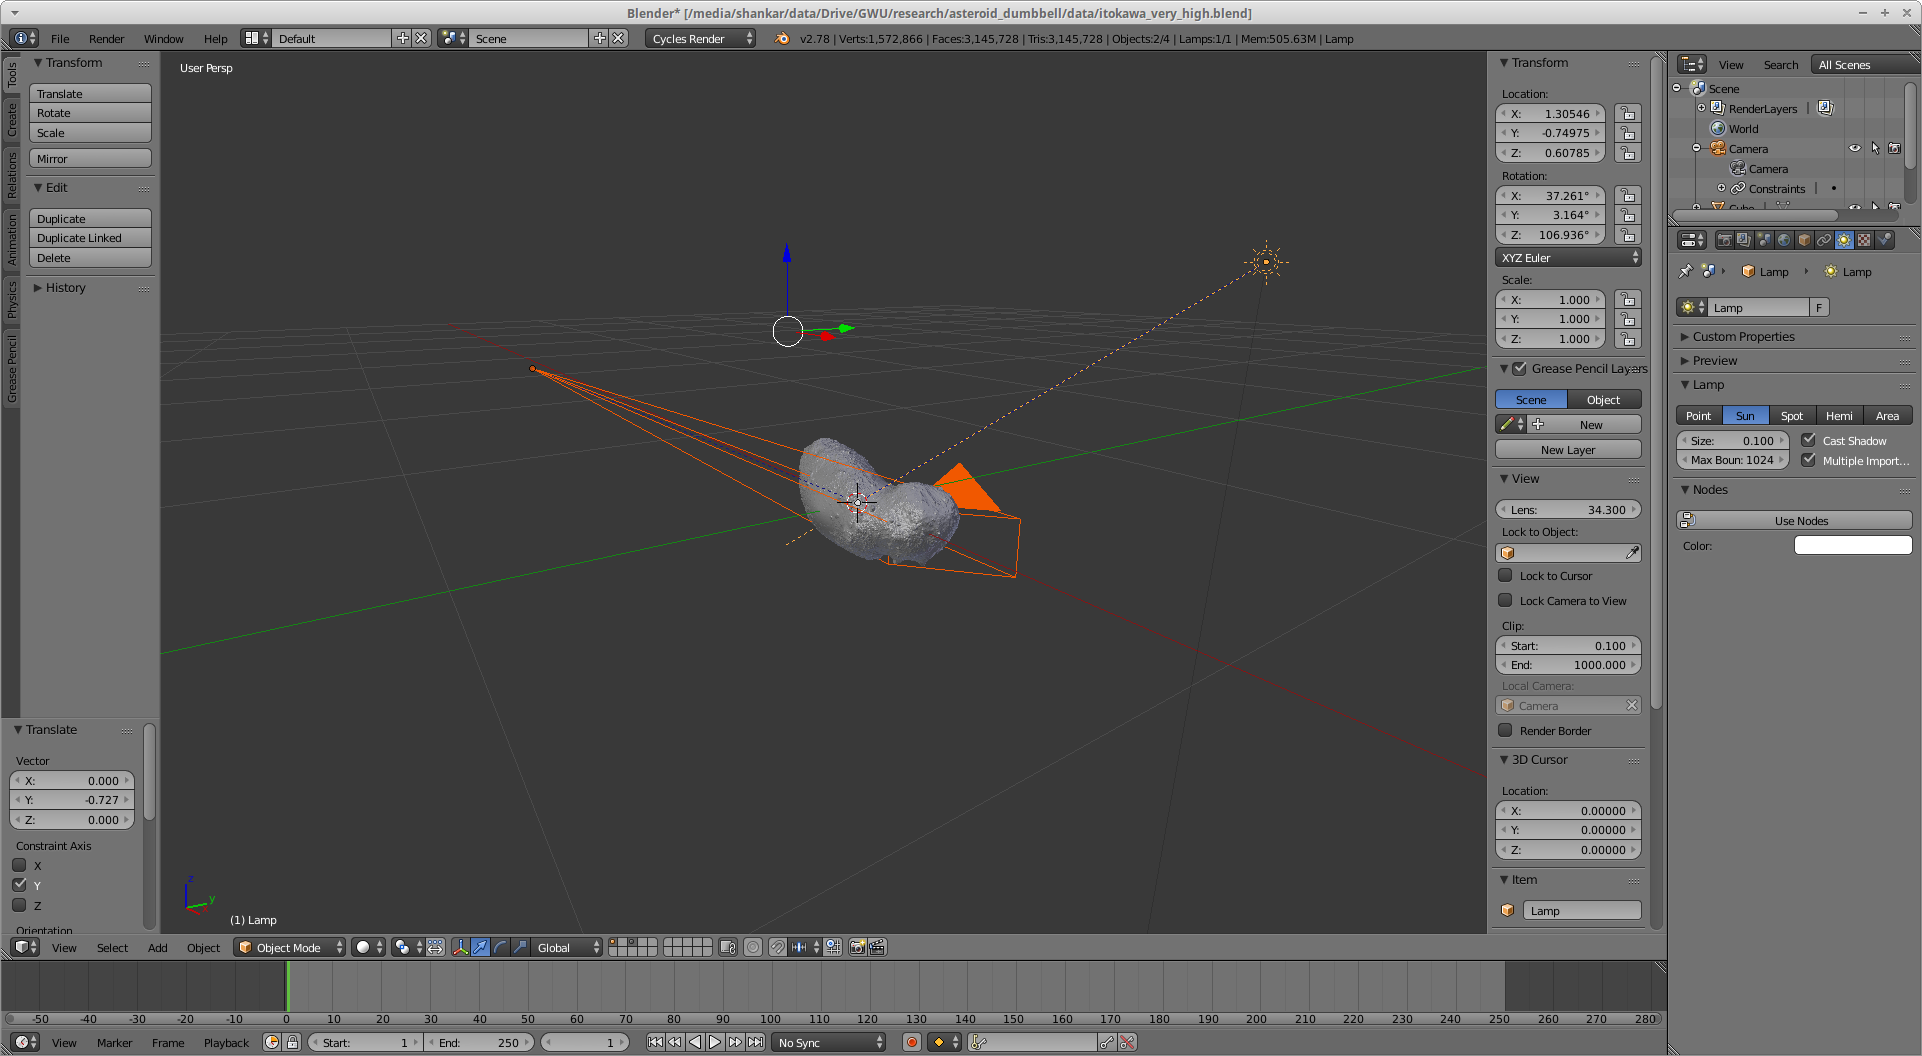
\includegraphics[width=0.8\columnwidth,height=0.4\textheight,keepaspectratio]{figures/2017AAS_asteroid_landing/blender_screenshot.png}\\
                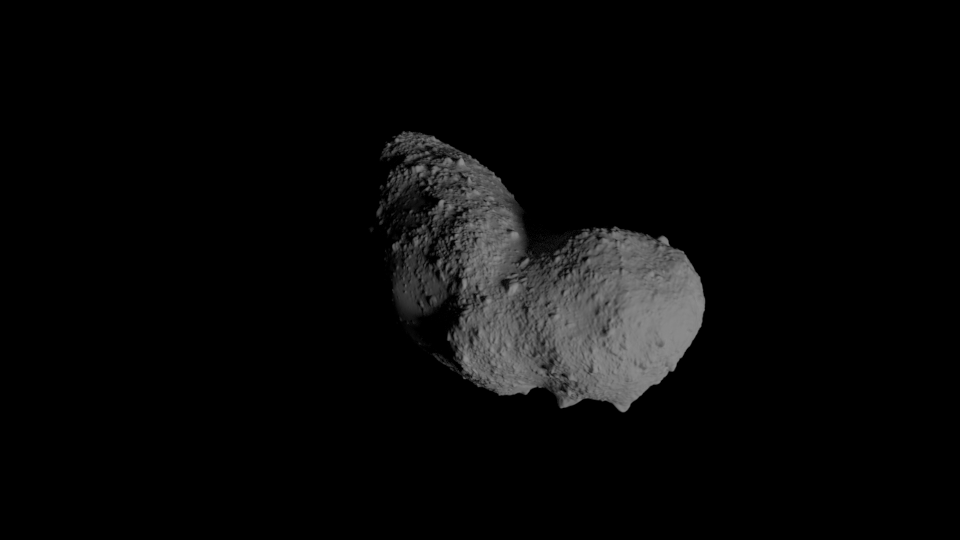
\includegraphics[width=0.8\columnwidth,height=0.4\textheight,keepaspectratio]{figures/2017AAS_asteroid_landing/itokawa_blender.png}
            \end{center}
        \end{column}
        \begin{column}{0.5\textwidth}
            \scriptsize
            \begin{semiverbatim}
            import bpy
    

            scene = bpy.context.scene

            bpy.ops.import\_scene.obj(`ast.obj')

            ast = bpy.data.objects[asteroid]


            ast.scale = [1, 1, 1] 

            ast.location = (0, 0, 0)
          

            scene.render.filepath = `out.png'

            bpy.ops.render.render(write\_still=True)

            \end{semiverbatim}
        \end{column}
    \end{columns}
}
\end{frame}

\begin{frame}[c]{Simulated imagery using Blender}
    \begin{itemize}
        \item Free \& open-source 3D computer graphics program
        \item Offer programmatic interface through Python
        \item Images of Itokawa emulated to match NEAR MSI camera
    \end{itemize}
    \begin{center}
        \animategraphics[controls,autoplay,loop,width=0.5\textwidth]{8}{animation/2017AAS_asteroid_landing/itokawa_landing/itokawa_landing_}{1}{1802}~
        \animategraphics[controls,autoplay,loop,width=0.5\textwidth]{8}{animation/2017AAS_asteroid_landing/itokawa_high/itokawa_high_}{1}{3000}~
    \end{center}
\end{frame}

\begin{frame}[c]{Monocular Localization}
    \begin{itemize}
        \item ORB-SLAM2 - Open-source mapping and localization framework
        \item Allows for real-time monocular based SLAM
        \item Utilized here to demonstrate localization from imagery
    \end{itemize}
    
    \begin{center}
        \animategraphics[controls,autoplay,loop,width=0.5\textwidth]{8}{animation/2017AAS_asteroid_landing/mappoints/mappoints_}{1}{1452}~
        \animategraphics[controls,autoplay,loop,width=0.5\textwidth]{8}{animation/2017AAS_asteroid_landing/local_crop/local_crop_}{1}{1452}~
    \end{center}
\end{frame}
